\documentclass{beamer}
\usepackage{beamerthemesplit}
\usepackage{wrapfig}
\usetheme{SPbGU}
\usepackage{pdfpages}
\usepackage{amsmath}
\usepackage{cmap} 
\usepackage[T2A]{fontenc} 
\usepackage[utf8]{inputenc}
\usepackage[english]{babel}
\usepackage{indentfirst}
\usepackage{amsmath}
\usepackage{tikz}
\usepackage{multirow}
\usepackage[noend]{algpseudocode}
\usepackage{algorithm}
\usepackage{algorithmicx}
\usetikzlibrary{shapes,arrows}
%usepackage{fancyvrb}
%\usepackage{minted}
%\usepackage{verbments}


\beamertemplatenavigationsymbolsempty

\title[Parsing techniques for graph analysis]{Parsing techniques for graph analysis}
%\subtitle[YaccConstructor]{Parsing techniques for graph analysis}
% То, что в квадратных скобках, отображается в левом нижнем углу. 
\institute[SPbU]{
JetBrains Research, Programming Languages and Tools Lab  \\
Saint Petersburg University
}

% То, что в квадратных скобках, отображается в левом нижнем углу.
\author[Ekaterina Verbitskaia]{Ekaterina Verbitskaia}

\date{Oktober 22, 2017}

\definecolor{orange}{RGB}{179,36,31}

\begin{document}
{
\begin{frame}[fragile]
  \begin{tabular}{p{3.5cm} p{5.5cm} p{1cm}}
   \begin{center}
      
\includegraphics[height=1.5cm]{pictures/jetbrainsResearch.pdf}
    \end{center}
    &
    \begin{center}
      
\includegraphics[height=1.5cm]{pictures/SLELogo.png}
    \end{center}
    &
    \begin{center}
      
\includegraphics[height=1.5cm]{pictures/SPbGU_Logo.png}
    \end{center} 
  \end{tabular}
  \titlepage
\end{frame}
}

\begin{frame}[fragile]
  \transwipe[direction=90]
  \frametitle{Language-constrained paths filtering}
  \begin{itemize}
    \item Can this automata generates SQL queries?
    \item Is there anybody one level above me in this hierarchy? 
  \end{itemize}
\end{frame}


\begin{frame}[fragile]
  \transwipe[direction=90]
  \frametitle{Language-constrained paths filtering: more formal}
  \begin{itemize}
    \item $\mathbb{G} = (\Sigma, N, P)$ --- context-free grammar
    \item $G = (V,E,L)$ --- directed graph, $E \subseteq V\times L \times V$, $L\subseteq \Sigma$
    \item $p=(v_0,l_0,v_1),\cdots,(v_{n-1},l_{n-1},v_n)$ --- path in $G$
    \item $\omega(p) = \omega((v_0,l_0,v_1),\cdots,(v_{n-1},l_{n-1},v_n)) = l_0 l_1 \cdots l_{n-1}$
    \item $R = \{ p | \exists N_i \in N (\omega(p) \in L(\mathbb{G},N_i))\}$
  \end{itemize}
\end{frame}

\begin{frame}[fragile]
  \transwipe[direction=90]
  \frametitle{Applications}
  \begin{itemize}
    \item Graph analysis
    \begin{itemize}
      \item Graph database querying
      \item Network graph analysis
      \item  
    \end{itemize}
    \item Сode analysis
    \begin{itemize}
      \item Static analysis CFL(linear conjunctive) reachability: alias analysis, points-to analysis, etc
      \item Dynamically generated strings analysis
      \item Multiple input parsing 
    \end{itemize}
    \item ...
  \end{itemize}
\end{frame}

\begin{frame}
  \transwipe[direction=90]
  \frametitle{Existing solutions}
  \begin{itemize}
    \item Graph data bsaes
    \item CFL-reachability
    \item 
  \end{itemize}
\end{frame}

\begin{frame}
  \transwipe[direction=90]
  \frametitle{Open problems}
  \begin{itemize}
    \item Effective algorithm creation
    \item Result representation for debugging, further processing 
    \item GPGPU utilization
  \end{itemize}
\end{frame}

\begin{frame}
  \transwipe[direction=90]
  \frametitle{Bar-Hillel theorem}
  \begin{itemize}
    \item Context-free languages are closed under intersection with regular languages
    \item Parsing algorithms are constructive proof of Bar-Hille theorem for one simple case ...
    \item ....so, it can be generalized for arbitrary regular language processing
  \end{itemize}
\end{frame}

\begin{frame}
  \transwipe[direction=90]
  \frametitle{Example}
\begin{figure}[ht]
    \centering
        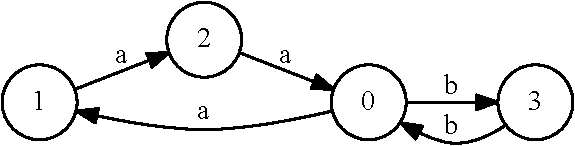
\includegraphics[width=0.45\textwidth]{pictures/input.pdf}
        \caption{An example: the map of School (input graph $M$)}
\end{figure}
\begin{figure}[ht]
\centering
   \[
\begin{array}{rl} 
   0:& S \rightarrow a \ S \ b \\
   1:& S \rightarrow Middle \\
   2:& Middle \rightarrow a \ b
\end{array}
\]
   \caption{An example: grammar $G_1$ for language $L=\{a^n b^n; n \geq 1\}$ with additional marker for the middle of a path}
   \label{grammarG}        
    \end{figure}
\end{frame}

\begin{frame}
  \transwipe[direction=90]
  \frametitle{Example}
\begin{figure}[ht]
    \centering
        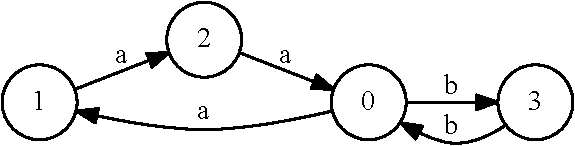
\includegraphics[width=0.45\textwidth]{pictures/input.pdf}
        \caption{An example: the map of School (input graph $M$)}
\end{figure}

\begin{tabular}{  c  c  c  }
      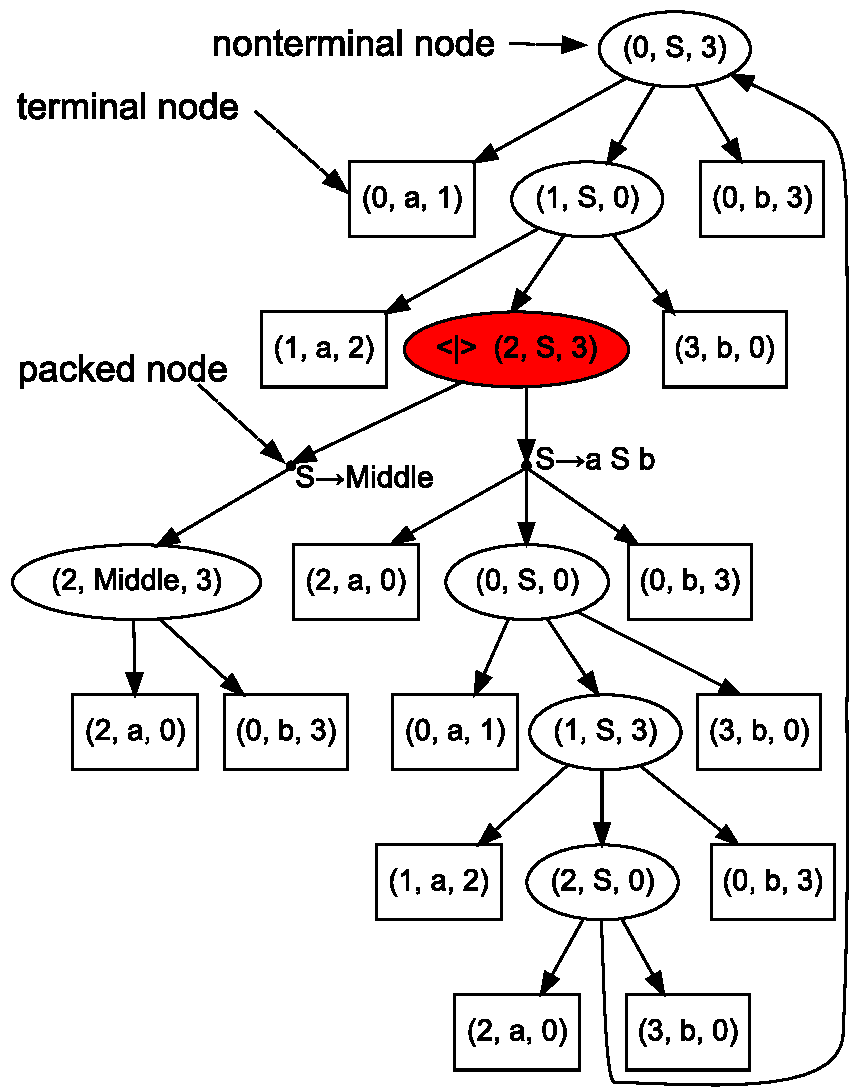
\includegraphics[height=4.5cm]{pictures/AnBn.pdf}
    &
      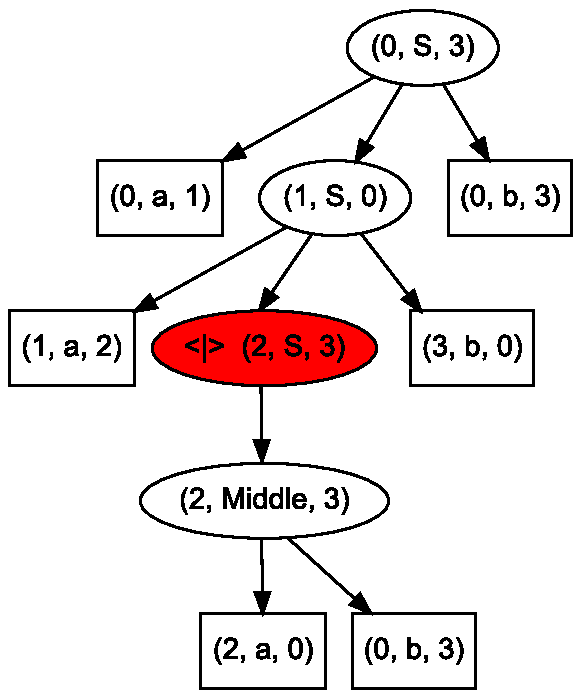
\includegraphics[height=4.5cm]{pictures/AnBn_2.pdf}
    &
      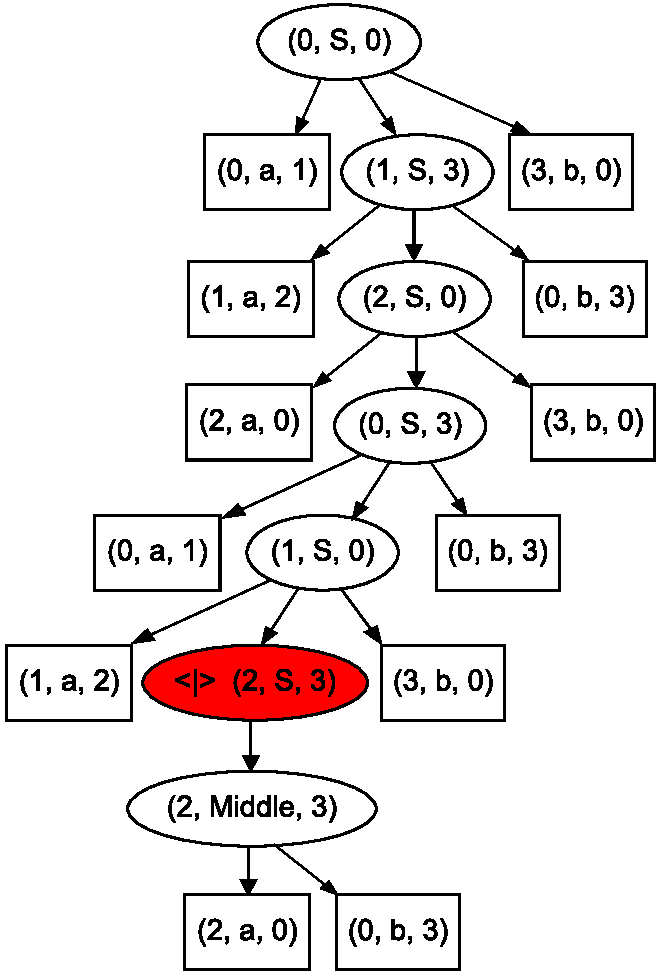
\includegraphics[height=4.5cm]{pictures/AnBn_1.pdf}

\\
sppf
& дерево
& дерево
  \end{tabular}
\end{frame}


\begin{frame}
  \transwipe[direction=90]
  \frametitle{Our solutions}
  \begin{itemize}
    \item Relaxed parsing of dynamically generated SQL-queries.
    \begin{itemize}
        \item Based on RNGLR parsing algorithm (Izmailova, Afroozeh)
    \end{itemize}
    \item Context-free path querying with structural representation of result.
    \begin{itemize}
        \item Based on GLL parsing algorithm (Izmailova, Afroozeh)
    \end{itemize}
    \item Combinators for context-free path querying
    \begin{itemize}
        \item Based on Meerkat (Izmailova, Afroozeh)
    \end{itemize}
    \item Context-free path querying by matrix multiplication
    \begin{itemize}
        \item Inspired by Valiant and Okhotin
    \end{itemize}
  \end{itemize}
\end{frame}

\begin{frame}[fragile]
\transwipe[direction=90]
\frametitle{Future work}
\begin{itemize}
  \item Other grammars and language classes intersection
  \begin{itemize}
     \item Context-free grammars intersection: Mark-Jan Nederhof, ``The language intersection problem for non-recursive context-free grammars''
     \item Approximated intersection of regular and conjunctive/boolean languages
     \item ...
  \end{itemize}
  \item Mechanization in Coq
  \begin{itemize}
     \item Bar-Hillel theorem
     \item GLL-based algorithms
     \item ...
  \end{itemize}
  \item New areas for application
\end{itemize}
\end{frame}
            
\begin{frame}
\transwipe[direction=90]
\frametitle{Information}
\begin{itemize}
  \item Ekaterina Verbitskaia: \href{mailto:kajigor@gmail.com}{kajigor@gmail.com}
  \item Semyon Grigorev: \href{mailto:semen.grigorev@jetbrains.com}{semen.grigorev@jetbrains.com}
  \item YaccConstructor: \href{https://github.com/YaccConstructor}{https://github.com/YaccConstructor}
\end{itemize}
\end{frame}
\end{document}
